%Matteo Kumar - Leonard Schatt
% Fortgeschrittenes Physikalisches Praktikum
 
\section{Absorption}\label{sec:Q3}
Absorption of monochromatic radiation can be described using the Lambert-Beer-law
\begin{equation}
    I(d) = I_0 \exp[-\mu d\rho],
\end{equation}
with the transmitted intensity $I$ as a function of the thickness of the material $d$, its density $\rho$, the mass attenuation coefficient $\mu$ and the incoming intensity $I_0$~\cite{Bohm.2021}. Differing from this law, an absortion spectrum shows discontinuities, called absorption edges (FIG). They were first explained by W.~Kossel as result of an incoming photon having exact the ammount of energy needed to excite an electron to a higher energy level, which leads to a instantaneous higher rate of absorption~\cite{Kossel.1920}. A display of the mass attenuation coefficient can be seen in Fig.~\ref{fig:muAbs}.

\begin{figure}[ht]
    \centering
    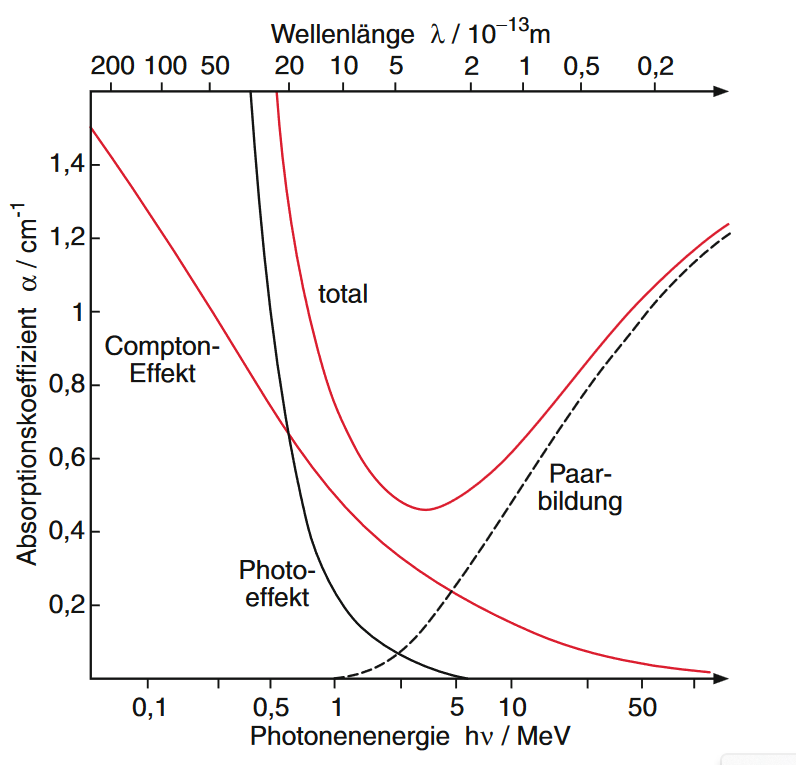
\includegraphics[width = 0.6\textwidth]{Bilder/Grundlagen/MuAbs.png}
    \caption{Mass attenuation coefficient $\alpha$ as function of the wavelength $\lambda$ or the photon energy $h\nu$. $\alpha$ depends on the strength of the influences of the photoelectric effect, the Compton effect and the $e^+$-$e^-$-pair-generation. Figure from \cite{Demtroeder.2016}}
    \label{fig:ConcReflTrans}
\end{figure}